\documentclass[12pt,letterpaper]{article}
\usepackage[top=1.5 in, bottom = 1.5 in, left = 1 in, right=1 in]{geometry}
\usepackage[american]{babel}
\usepackage[numbers]{natbib}
\usepackage{etoolbox}
\apptocmd{\thebibliography}{\raggedright}{}{}
\usepackage{amsmath}
\usepackage{amssymb, amsfonts, textcomp}
\usepackage{titlesec}
\usepackage{color}
\usepackage{multicol}
\usepackage{multirow}
\usepackage{tabu}
\usepackage{booktabs}
\usepackage{array}
\usepackage{hhline}
\usepackage{hyperref}
\usepackage{fontspec}
\setmainfont{Chaparral Pro}
\setromanfont{Chaparral Pro}
\setmonofont{Consolas}
\setsansfont{Myriad Pro}
\setcounter{secnumdepth}{5}
\pagestyle{plain}
\addto\captionsamerican{ %babel
	\renewcommand\contentsname{Table of Contents}
}
\renewcommand\thesection{\arabic{section}}
\renewcommand\thesubsection{\arabic{section}.\arabic{subsection}}
\renewcommand\thesubsubsection{\arabic{section}.\arabic{subsection}.\arabic{subsubsection}}
\renewcommand\theparagraph{\arabic{section}.\arabic{subsection}.\arabic{subsubsection}.\arabic{paragraph}}
\renewcommand\thesubparagraph{\arabic{section}.\arabic{subsection}.\arabic{subsubsection}.\arabic{paragraph}.\arabic{subparagraph}}

%\titleformat{<command>}[<shape>]{<format>}{<label>}{<sep>}{<before-code>}[<after-code>]
\titleformat{\subparagraph}[hang]
{\normalfont\normalsize\bfseries}{\thesubparagraph}{1 em}{}[]
%\titlespacing*{<command>}{<left>}{<before-sep>}{<after-sep>}
\titlespacing*{\subparagraph}{0 pt}{2 ex}{.25 ex}

\titleformat{\paragraph}[hang]
{\normalfont\normalsize\bfseries}{\theparagraph}{1 em}{}[]
\titlespacing*{\paragraph}{0 pt}{2 ex}{.25 ex}

\begin{document}
	\pagenumbering{gobble}
	\vspace*{2.8 in}
	\begin{huge}
		\begin{center}
			Software Project Management Plan
			\par
			for
			\par
			The Walking Game
			\par
		\end{center}
	\end{huge}
	\vspace*{2.5 in}
	\begin{large}
		\begin{flushright}
			Star Team
			
			Version: 1.1
			
			Date: 10/31/2014
		\end{flushright}
	\end{large}
	
	\clearpage
	\section*{Revision History}
	\begin{flushleft}
		\begin{tabular}{|p{0.855in}|p{0.8in}|p{2.7in}|p{1.298in}|}
			\hline
			\textbf{Revision \#} & \textbf{Date} & \textbf{Description} & \textbf{Author} \\\hline
			1.0 & 10/29/2014 & Initial revision & Samuel I. Gunadi \\\hline
			1.1 & 10/31/2014 & Improved typesetting and added project website URL & Samuel I. Gunadi \\\hline
		\end{tabular}
	\end{flushleft}
	\clearpage
	\bigskip
	\tableofcontents
	
	\clearpage
	\bigskip
	\listoftables
	
	\clearpage
	\bigskip
	\listoffigures
	
	\clearpage
	\setcounter{page}{0}
	
	\pagenumbering{arabic}
	\section{Introduction}
	The Software Project Management Plan for The Walking Game project defines the project management goals of the project and includes a description of the deliverables and deadlines. Star team consists of: Samuel I. Gunadi, Roberto J. Kondurura, and Ryan Elegant. Star team has a goal to fulfill the requirements of the software engineering course at Universitas Pelita Harapan.
	
	\subsection{Project Overview}
	This section of the Software Project Management Plan (SPMP) gives an overview of the purpose, scope, and objectives of the project. It also contains sections regarding the assumptions and constraints, the project deliverables, the summary of the schedule, and the plan for change in the SPMP.
	
	\subsubsection{Purpose, scope and objective}
	This project aims to educate and entertain users---educate, by studying the source code, and entertain, by playing and interacting through the console. This project will mostly benefits the team as part of their Computer Graphics and Software Engineering course assignments.
	
	The project will have a Wavefront OBJ file parser; people 3D models, textures, and walking animations; textures with alpha blending; a textured floor; collision detection; simple command interpreter and scripting; nameplates; and an MMORPG style third-person camera. The project website can be found at \begin{footnotesize}\url{https://github.com/samuelgunadi/thewalkinggame}\end{footnotesize}.
	
	\subsubsection{Assumptions and Constraints}
	There are several assumptions and constraints that are important for the project and its team members.
	
	\paragraph{Assumptions}
	The assumptions are as follows:
	
	•\enspace The team consists of 3 people and additional human resources will not be available.
	
	•\enspace The team is experienced enough to complete the project.
	
	•\enspace The team will work together to complete the project
	
	
	\paragraph{Constraints}
	The constraints are as follows:
	
	•\enspace The team members' time on the project will be limited to approximately 5 hours per week.
	
	•\enspace The budget is US\$ 0 and additional financial resources are not available for the project.
	
	
	\subsubsection{Project Deliverables}
	
	The Star team will deliver a working system that satisfies the requirements.
	
	\paragraph{Software Deliverables}
	
	The Star team will deliver the software program and its third-party libraries.
	
	\paragraph{Documents Deliverables}
	
	Documentation will be delivered by the Star team during the course of the project. Some of the documents are intended for team use and are required by the Software Engineering course, while other documents are part of the deliverable to the client.
	
	
	\subparagraph{Team Documents}
	
	The following documents are for the team use and are required by the Software Engineering course:
	
	•\enspace Software Project Management Plan (SPMP)
	
	•\enspace Software Requirement Specification (SRS)
	
	
	\subparagraph{Client Documents}
	The following documents will be delivered to the client: 
	•\enspace Installation documentation
	
	•\enspace End-user documentation
	
	
	\subsubsection{Schedule}
	The schedule of the project phases, milestones and corresponding documents is given in Table \ref{tab:t1}.
	
	\begin{table}[h]
		\begin{tabular}{|p{2.28 in}|p{2.6 in}|p{1.05 in}|}
			\hline
			{\bfseries Project milestone} & {\bfseries Project artifact} & {\bfseries Due date} \\\hline
			Project start                 &                              & 08/10/2014 \\\hline
			Producing needed documents    & SPMP and SRS                 & 09/24/2014 \\\hline
			Phase 1 completion            & Phase 1 delivery             & 10/14/2014 \\\hline
			Phase 2 completion and final presentation & Phase 2 delivery and user documentation & 11/19/2014 \\\hline
		\end{tabular}
		\caption{Star team's Milestones and due date}
		\label{tab:t1}
	\end{table}
	
	\subsection{Evolution of the SPMP}
	The SPMP for The Walking Game project will be under version control Git, so any changes will be made to the plan itself. The updated document will be made available to all project members and interested stakeholders on the project's web site \begin{footnotesize}\url{https://github.com/samuelgunadi/thewalkinggame}\end{footnotesize}.
	
	\nocite{*}
	
	\begingroup
		\section{References}
		\renewcommand{\section}[2]{}%
		\bibliographystyle{IEEEtranN}
		\bibliography{references}
	\endgroup
	
	\clearpage
	\section{Definitions}
	SPMP --- Software Project Management Plan
	
	\vspace{0.1in}\noindent SRS --- Software Requirements Specification
	
	\vspace{0.1in}\noindent VM --- Virtual Machine
	
	\vspace{0.1in}\noindent OpenGL --- Open Graphics Library
	
	\vspace{0.1in}\noindent PDF --- Portable Document Format
	
	\vspace{0.1in}\noindent IDE --- Integrated Development Environment
	
	\clearpage
	\section{Project Organization}
	This SPMP will identify the organizational entities external to the project and their interaction with the project team, as well as internal project structure and roles and responsibilities for the project. 
	
	\subsection{External Structure}
	The clients for this project are David Hareva, Star team's computer graphics lecturer and Robertus Hudi, Star team's software engineering assistant lecturer. The Star team communicates with the client at each class meeting.
	
	\subsection{Internal Structure}
	\begin{figure}[h]
		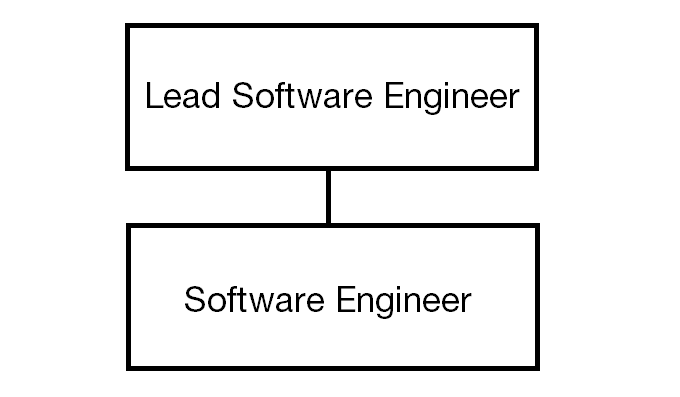
\includegraphics[width=6.5in,height=3.79in]{fig_1.png} 
		\caption{Internal team structure}
		\label{fig:f1}
	\end{figure}
	
	The team structure is hierarchical. Figure \ref{fig:f1} shows the internal team structure, consisting of 2 roles.
	
	\clearpage
	\bigskip
	
	\subsection{Roles and Responsibilities}
	Star team's roles and respective responsibilities are shown in Table \ref{tab:t2}.
	
	\begin{table}[h]
		\begin{flushleft}
			\begin{tabular}{|p{1.73in}|p{4.3in}|}
				\hline
				Role &
				Responsibilities\\\hline
				Lead Software Engineer &
				•\enspace Motivate the team members to perform their tasks
				
				•\enspace Help the team in allocating the tasks and resolving issues
				
				•\enspace Create and maintain SPMP
				
				•\enspace Create, develop, and maintain SRS
				
				•\enspace Establish and maintain the team's development standards
				
				•\enspace Lead the team in implementing the product
				
				•\enspace Lead the team in developing the tests and running the tests
				
				\\\hline
				Software Engineer &
				•\enspace Implement the product
				
				•\enspace Develop and run tests
				
				•\enspace Produce user documentation
				
				\\\hline
			\end{tabular}
		\end{flushleft}
		\caption{Star team's roles and respective responsibilities}
		\label{tab:t2}
	\end{table}
	
	\clearpage
	\bigskip
	
	\section{Managerial Process}
	\subsection{Work Plan}
	The SPMP will specify the work activities, schedule and resources for The Walking Game project.
	
	\subsubsection{Work lists}
	Table \ref{tab:t3} and Figure \ref{fig:f2} outlines the major work activities and their dependencies for the duration of the project.
	
	\begin{table}[h]
		\begin{flushleft}
			\begin{tabular}{|p{0.306 in}|p{0.594 in}|p{2.758 in}|p{0.9177 in}|p{0.917 in}|}
				\hline
				ID & WBS & Task Name & Start Date & Finish Date \\\hline
				1 & 1 & Education and requirements phase & 08/10/2014 & 08/24/2014 \\\hline
				2 & 1.1 & OpenGL and content creation tools education & 08/10/2014 & 08/24/2014 \\\hline
				3 & 1.2 & Requirements phase & 08/10/2014 & 09/24/2014 \\\hline
				4 & 1.2.1 & Requirements gathering & 08/10/2014 & 08/24/2014 \\\hline
				5 & 1.2.2 & Requirements analysis & 08/24/2014 & 09/10/2014 \\\hline
				6 &
				1.2.3 & SRS preparation & 09/10/2014 & 09/24/2014 \\\hline
				8 & 2 & SPMP document preparation & 08/10/2014 & 08/24/2014 \\\hline
				9 & 3 & Phase 1 & 11/01/2014 & 10/14/2014 \\\hline
				10 & 4 & Phase 2 & 10/15/2014 & 11/18/2014 \\\hline
				11 & 5 & Final presentation & 11/19/2014 & 11/19/2014 \\\hline
			\end{tabular}
		\end{flushleft}
		\caption{Overall project plan}
		\label{tab:t3}
	\end{table}
	
	\begin{figure}[h]
		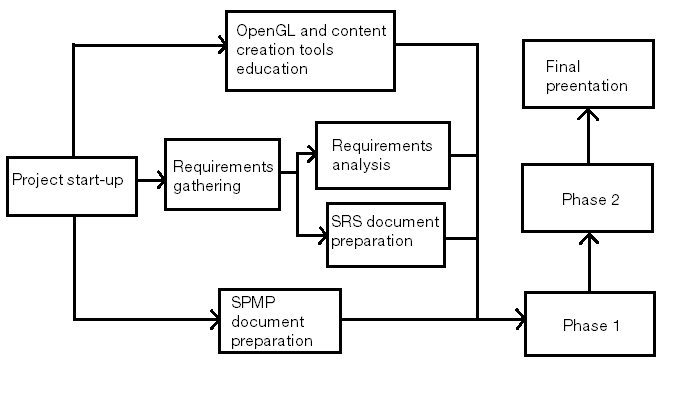
\includegraphics[width=6.5in,height=3.79in]{fig_2.png} 
		\caption{Project activity network diagram}
		\label{fig:f2}
	\end{figure}
	
	\clearpage
	\bigskip
	
	\section{Technical Process}
	The SPMP will specify the development process model, technical models, tools and techniques that will be used to develop the work products, project infrastructure and product acceptance plan.
	
	\subsection{Process Model}
	The Walking Game project will follow an incremental and an iterative development model for its deliverables. The development will be done in several phases and each phase will represent a complete development cycle, with certain functionality of the system delivered at the end of each phase. The phased approach to delivery provides flexibility in what the team will deliver, gives an opportunity to reassess the effort for each phase and allows both the team and the client to change any of the phase's content. The project phases are outlined in Table \ref{tab:t4}.
	
	\begin{flushleft}
		\begin{table}[h]
			\begin{tabular}{|p{1.23in}|p{1.233in}|p{3.49in}|}
				\hline
				Phase & Start and finish date & Phase goals \\\hline
				Project start-up and learning &	10/10/2014 to 10/31/2014 &
				1. Task allocation
				\par
				2. Learn OpenGL and related tools
				\par
				3. Learn 3D content creation tools \\\hline
				Requirements &
				10/11/2014 to 10/21/2014 &
				1. Become familiar with requirements
				\par
				2. Create and review the required documents \\\hline
				Phase 1 &
				11/01/2014 to 11/15/2014 &
				1. Implement a Wavefront OBJ parser
				\par
				2. Create 3D models
				\par
				3. Create textures
				\par
				4. Create animation \\\hline
				Phase 2 &
				11/16/2014 to 11/30/2014 &
				1. Implement collision handler
				\par
				2. Implement console commands interpreter
				\par
				3. Implement third-person camera
				\par
				4. Implement character controls
				\par
				5. Implement nameplates \\\hline
			\end{tabular}
			\caption{The Walking Game project phases and goals}
			\label{tab:t4}
		\end{table}
	\end{flushleft}
	
	\subsection[Methods, Tools, and Techniques]{Methods, Tools, and Techniques}
	The Star team uses object-oriented methodology and software patterns. Microsoft Visual Studio is used as primary IDE, with Microsoft Visual C++ Compiler the compiler. The programming languages used are C++ and C. Autodesk Maya, Autodesk 3dsMax, Autodesk Mudbox, DAZ3D Studio, Pixologic ZBrush, and Adobe Photoshop are used as the content creation tools. Git is be used for revision control. Documentation is created using Latex which is then compiled into PDF documents.

	\subsection{Infrastructure Plan}
	The Star team has three Windows computers available for this project. The team also has access to
	Linux VM and a printer.
\end{document}